\chapter{Results}

\subsection{15.11 Preliminary Results}

Table 15.1 presents the baseline model performance on the stationary validation set (75,000 flows) extracted directly from results/model\_comparison.csv. XGBoost achieved the highest ROC-AUC (0.9228) and lowest error count (753 errors) and was selected as the operational classifier.

\begin{table}[H]
\centering
\small
\begin{tabular}{p{0.15\textwidth} p{0.15\textwidth} p{0.15\textwidth} p{0.15\textwidth} p{0.15\textwidth} p{0.15\textwidth} p{0.15\textwidth}}
\toprule
\textbf{Model} & \textbf{Accuracy (\%)} & \textbf{Precision} & \textbf{Recall} & \textbf{F1-Score} & \textbf{Validation ROC-AUC} & \textbf{Val Errors} \\
\midrule
Logistic Regression & 96.06\% & 0.0376 & 0.4435 & 0.0693 & 0.7499 & 2,953 \\
Random Forest & 98.01\% & 0.0708 & 0.4153 & 0.1210 & 0.8526 & 1,496 \\
XGBoost (Selected) & 98.996\% & 0.0401 & 0.0887 & 0.0552 & 0.9228 & 753 \\
\bottomrule
\end{tabular}
\caption{15.11 Preliminary Results}
\end{table}

Table 15.2 provides the definitive comparative benchmark across all five review allocation strategies on the 75,000 shifted test instances (3,427 total errors), extracted directly from results/final\_shifted\_strategy\_comparison.csv.

\begin{table}[H]
\centering
\small
\begin{tabular}{p{0.14\textwidth} p{0.16\textwidth} p{0.14\textwidth} p{0.18\textwidth} p{0.28\textwidth}}
\toprule
\textbf{Allocation Strategy} & \textbf{1\% Budget (K=750)} & \textbf{2\% Budget (K=1500)} & \textbf{5\% Budget (K=3750)} & \textbf{10\% Budget (K=7500)} \\
\midrule
Random Guessing (Baseline) & 1.17\% (40 errors) & 2.13\% (73 errors) & 5.52\% (189 errors) & 9.92\% (340 errors) \\
OOD Only (Mahalanobis Distance) & 0.03\% (1 error) & 0.26\% (9 errors) & 0.35\% (12 errors) & 0.35\% (12 errors) \\
Confidence Only (1 - Confidence) & 13.51\% (463 errors) & 26.73\% (916 errors) & 65.45\% (2,243 errors) & 84.01\% (2,879 errors) \\
Static Multi-Factor (Equal Weights) & 17.51\% (600 errors) & 34.00\% (1,165 errors) & 54.57\% (1,870 errors) & 65.42\% (2,242 errors) \\
Adaptive Multi-Factor (Feedback-Adaptive) & 17.80\% (610 errors) & 34.26\% (1,174 errors) & 45.90\% (1,573 errors) & 52.35\% (1,794 errors) \\
\bottomrule
\end{tabular}
\caption{15.11 Preliminary Results}
\end{table}

\begin{figure}[H]
\centering
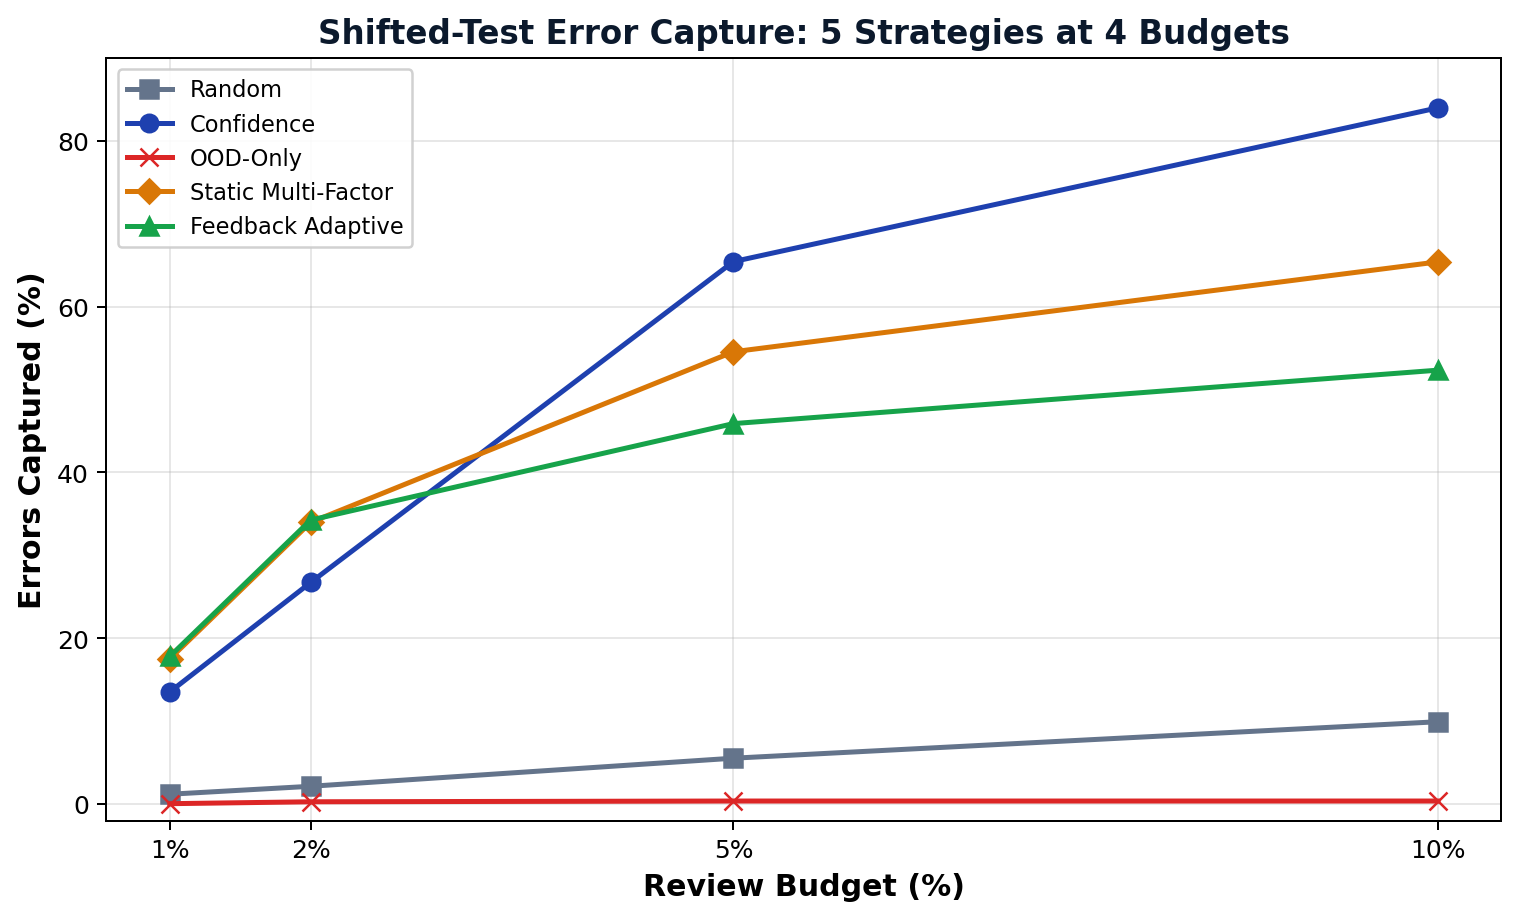
\includegraphics[width=0.85\textwidth]{figures/v2_results_chart.png}
\caption{Figure 15.1: Comparative Error Capture Rate Across Review Budgets (1\%--10\%).}
\end{figure}

\subsection{15.12 Analysis of Results}

\textbf{Key Findings \& Crossover Analysis:} The empirical benchmark results reveal three critical scientific findings regarding review allocation under temporal distribution shift:

\begin{itemize}
\item \textbf{1. Multi-Factor Advantage:} Multi-Factor Dominance at Tight Budgets (1\%--2\%): Under severe operational review constraints, the Adaptive Multi-Factor strategy captures 17.80\% of errors (610 errors) at a 1\% budget and 34.26\% (1,174 errors) at a 2\% budget---achieving an absolute improvement of +4.29\% and +7.53\% over pure confidence ranking (13.51\% and 26.73\%). This confirms that synthesizing drift and historical mistake proximity effectively catches high-confidence errors that bypass confidence filters.
\item \textbf{2. Honest Crossover:} The Budget-Dependent Crossover (5\%--10\%): At broader inspection budgets, a distinct performance crossover occurs: Confidence Only overtakes multi-factor allocation, capturing 65.45\% of errors at 5\% budget and 84.01\% at 10\% budget (versus 45.90\% and 52.35\% for Adaptive Multi-Factor). This occurs because XGBoost's probability distribution concentrates a large volume of errors in the moderate-confidence band (0.60--0.80), which confidence thresholding sweeps effectively at higher budgets.
\item \textbf{3. OOD Decoupling:} Poor Performance of Isolated OOD Detection in This Experiment (0.03\% to 0.35\%): OOD-only allocation captured only 1 error out of 3,427 at 1\% budget (0.03\%) and only 9 errors at 2\% budget (0.26\%), performing substantially worse than proportional random guessing (1.17\% and 2.13\%). In tabular network traffic under distribution shift, geometric feature distance measures benign feature variations (e.g., high-volume transfers) rather than classifier mistakes.
\end{itemize}

\begin{figure}[H]
\centering
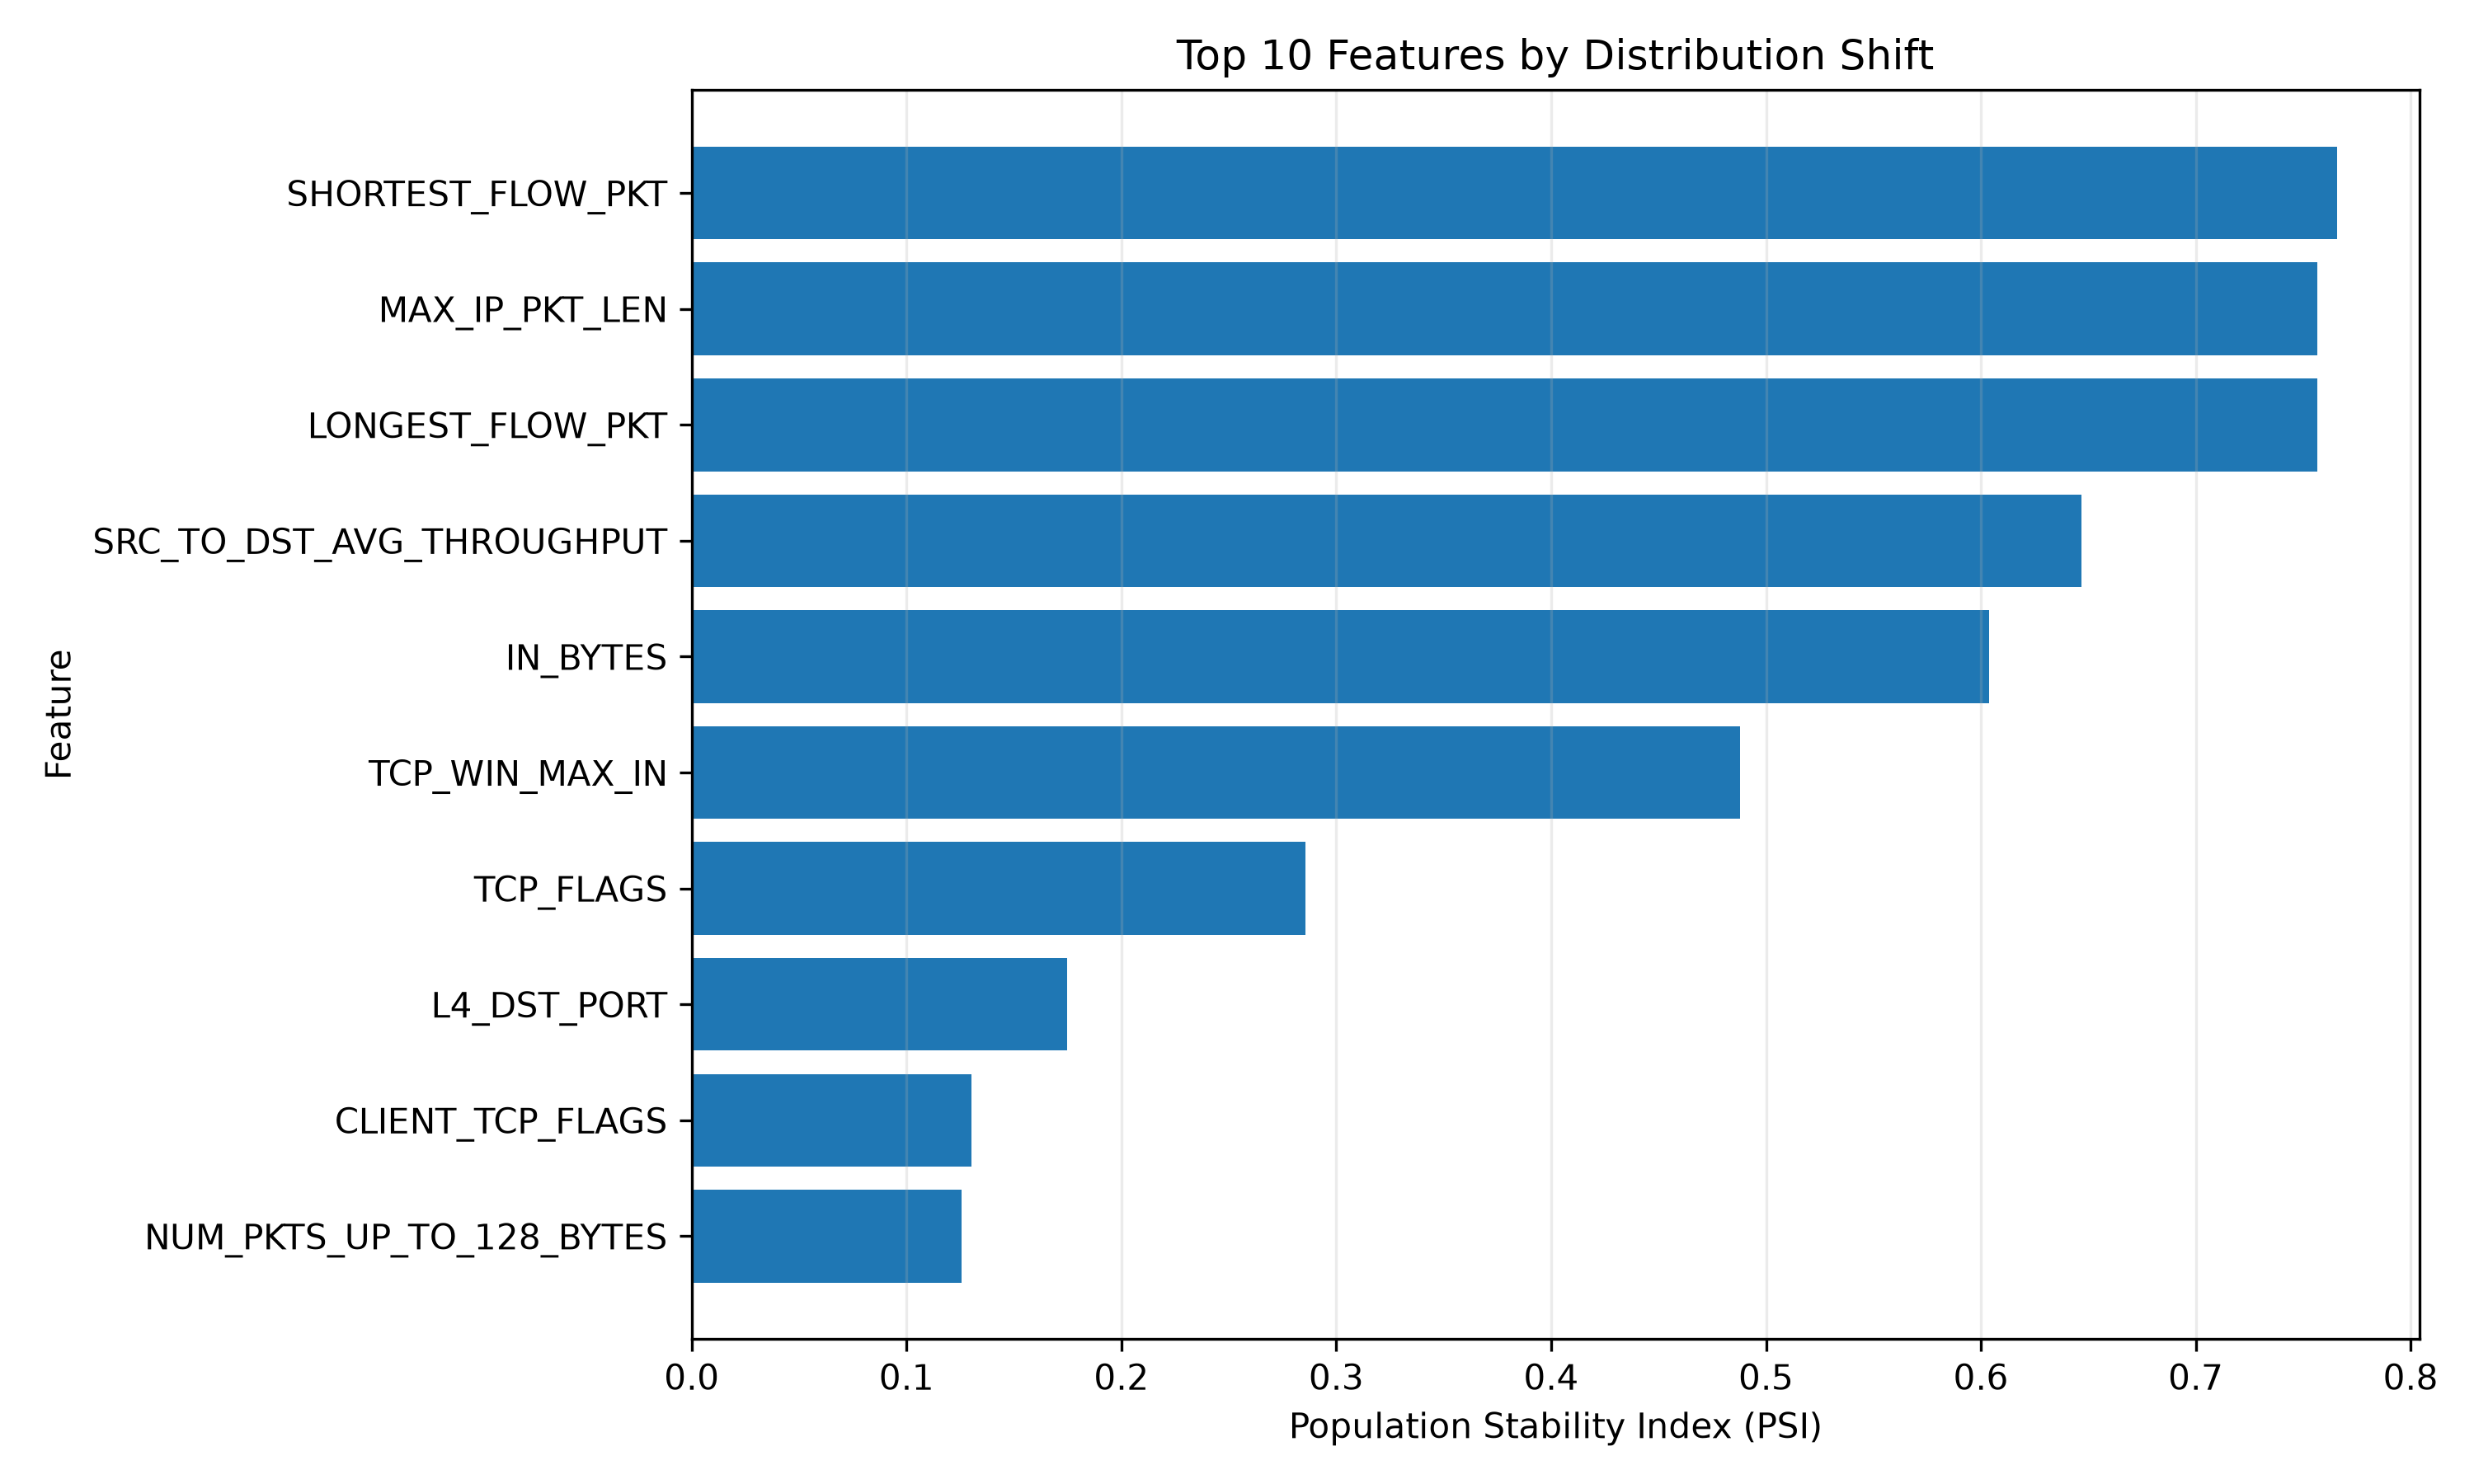
\includegraphics[width=0.85\textwidth]{figures/top10_drift_features.png}
\caption{Figure 15.2: Top 10 Features Exhibiting Highest Population Stability Index (PSI) Drift.}
\end{figure}

\begin{figure}[H]
\centering
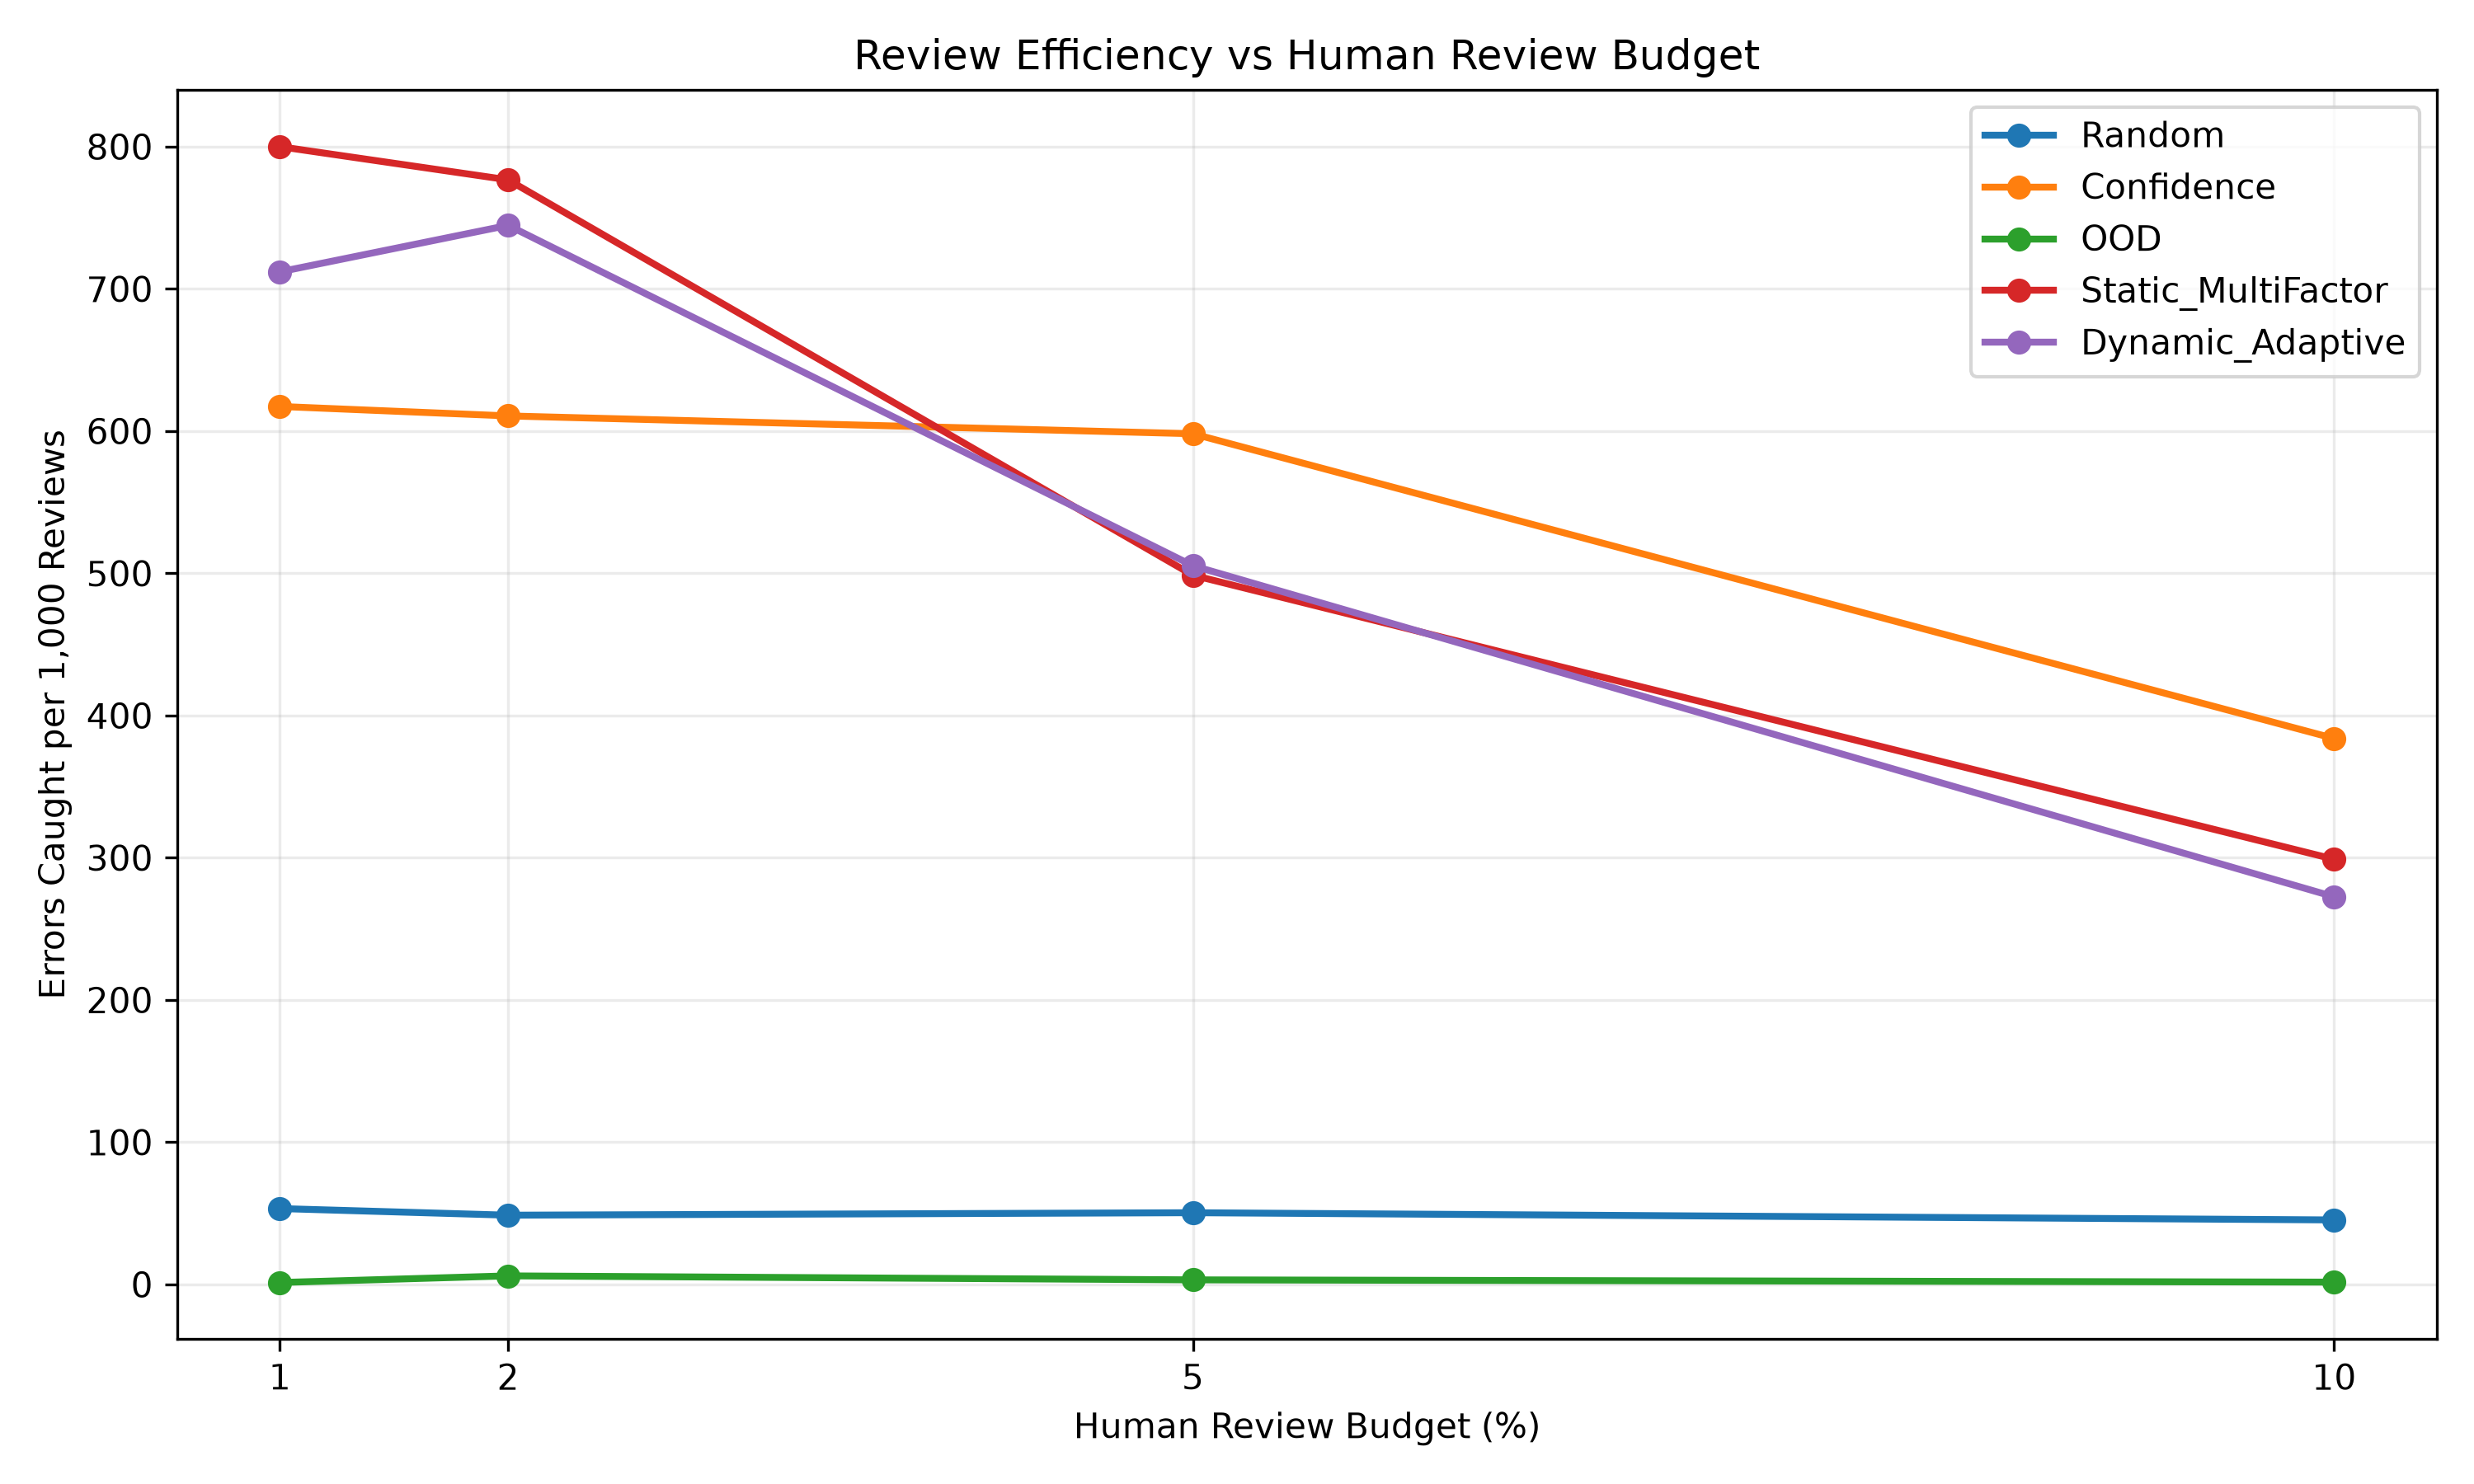
\includegraphics[width=0.85\textwidth]{figures/review_efficiency_vs_budget.png}
\caption{Figure 15.3: Review Efficiency (Precision of Review Queue) Across Allocation Budgets.}
\end{figure}

\section{Testing / Evaluation}

System verification encompasses functional unit testing, UI/UX responsiveness evaluation, and model shift validation.

\subsection{16.1 Functional Testing}

Table 16.1 outlines the functional test cases executed across the data pipeline, model inference service, and review queue allocation logic.

\begin{table}[H]
\centering
\small
\begin{tabular}{p{0.14\textwidth} p{0.16\textwidth} p{0.14\textwidth} p{0.18\textwidth} p{0.28\textwidth}}
\toprule
\textbf{Test ID} & \textbf{Module / Component} & \textbf{Test Scenario} & \textbf{Expected Outcome} & \textbf{Status} \\
\midrule
TC-01 & M1: Data Ingestion & Verify 500K records loaded with 55 raw attributes and correct SHA-256. & Matches reference checksum; zero missing rows. & PASSED \\
TC-02 & M1: Temporal Splitting & Enforce strict chronological sorting (350K train, 75K val, 75K test). & Train max timestamp < Val min timestamp < Test min. & PASSED \\
TC-03 & M2: Imputation & Impute nulls/inf values using training set medians. & Zero NaN values in preprocessed feature matrix. & PASSED \\
TC-04 & M3: Uncertainty Signal & Compute 1 - max(P, 1-P) across validation inferences. & Output bounded strictly in [0.0, 0.5]; higher for P \textasciitilde{} 0.5. & PASSED \\
TC-05 & M3: Mahalanobis OOD & Compute distance with Tikhonov regularization (eps = 1e-6). & Matrix inversion stable; distances converted to percentiles. & PASSED \\
TC-06 & M3: PSI Drift & Calculate PSI across 49 features over 10 quantile bins. & PSI correctly flags high-drift features (e.g., flow\_duration). & PASSED \\
TC-07 & M4: Budget Quota & Verify queue size equals exactly floor(B * N) for B in \{1\%, 2\%, 5\%, 10\%\}. & Exact allocation: 750, 1500, 3750, 7500 instances. & PASSED \\
TC-08 & M5: Feedback Loop & Adjust historical error weight based on audit error density. & Weights adapt dynamically and re-normalize to sum = 1.0. & PASSED \\
\bottomrule
\end{tabular}
\caption{16.1 Functional Testing}
\end{table}

\subsection{16.2 UI / UX Testing}

\textbf{Dashboard Usability:} The Streamlit analytics dashboard (dashboard/app.py) was tested across standard user workflows. The application launches locally in under 3.5 seconds, executes Plotly chart re-rendering in <120ms upon slider budget adjustment, and maintains stable memory usage (<350 MB) during multi-filter exploration.

\subsection{16.3 Model Evaluation}

\textbf{Distribution Shift Validation:} The shifted test period shows substantially higher classification error (surging 4.55x from 1.004\% on validation to 4.569\% on shifted test) while model confidence remains high, indicating reduced prediction reliability under temporal shift. The evaluation confirms that traditional static accuracy metrics fail to reflect operational degradation, proving the necessity of adaptive human-review safety filters.

